\documentclass[tikz]{standalone} %\usetikzlibrary{calc} 
\usepackage{rubikcube,rubikrotation,rubikpatterns,rubiktwocube} 
\newcommand{\CycleThreeEdgesFlipTwo}{[CycleThreeEdgesFlipTwo],F,R,U,Rp,Up,Fp}%
\newcommand{\cyclethreeedgesfliptwo}{\CycleThreeEdgesFlipTwo}%
\standaloneconfig{border=0bp}
%
%----corner sequences--------------------------
\newcommand{\AllYellow}{[allyellow],R,U,Rp,U,R,Up,Up,Rp}% = SUNE  %cross -->allyellow
\newcommand{\allyellow}{\AllYellow}%
\newcommand{\CycleThreeCorners}{[cyclethreecorners],Lp,U,R,Up,L,U,Rp,Up}%
\newcommand{\cyclethreecorners}{\CycleThreeCorners}%
\newcommand{\CornerRotation}{[CornerRotation],Up,Rp,Dp,R,U,Rp,D,R}
\newcommand{\cornerrotate}{[cornerrotate],Up,Rp,Dp,R,U,Rp,D,R}
\newcommand{\SwapTwoCorners}{[swaptwocorners],Rp,F,Rp,B2,R,Fp,Rp,B2,R2,Up}
\newcommand{\swaptwocorners}{\SwapTwoCorners}
\newcommand{\CornerOrientation}{[CornerOrientation],Rp,D2,R,Bp,U2,B,Rp,D2,R,Bp,U2,B} % (R^{-1} D^2 R B^{-1} U^2 B)^2
\newcommand{\EdgeOrientation}{[EdgeOrientation],Sr,U,Sr,U,Sr,U2,Srp,U,Srp,U,Srp,U2}
%
%% brace and bracket macros 
\newcommand{\Rubikbracket}[1]{$\left(\mbox{#1}\right)$}
\newcommand{\Rubikbrace}[1]{$\left\{\mbox{#1}\right\}$}
\newcommand{\cubenumber}[1]{\strut\raisebox{1cm}{#1}}
\definecolor{ptblue}{HTML}{2A5EA4}
\usepackage{amsmath, amssymb, multicol}
\usepackage{graphicx}
\usepackage{textcomp}
\usepackage{chessboard}

\def\d{\displaystyle}
\def\b{\mathbf}
\def\R{\mathbf{R}}
\def\Z{\mathbf{Z}}
\def\st{~:~}
\def\bar{\overline}
\def\inv{^{-1}}

\def\v{circle (3pt)}

\begin{document}
 % \begin{multicols}{4}




%    \begin{center}

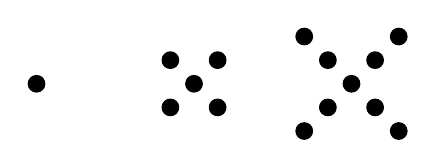
\begin{tikzpicture}
	\draw[fill = black] (-2,0) \v ;
    \draw[fill = black] (0,0) \v (.3, .3) \v (-.3,-.3) \v (-.3, .3) \v (.3,-.3) \v;
    \draw[fill = black] (2,0) \v (2.3, .3) \v (1.7, -.3) \v (1.7, .3) \v (2.3, -.3)\v (2.6, .6) \v (2.6, -.6) \v (1.4, .6) \v (1.4, -.6) \v;
    \end{tikzpicture}
%
%  $n = 0$
%  \end{center}
%
%
%  \columnbreak
%
%
%
%    \begin{center}
%    \begin{tikzpicture}
%    \draw[fill = black] (0,0) \v (.3, .3) \v (-.3,-.3) \v (-.3, .3) \v (.3,-.3) \v;
%    \end{tikzpicture}
%
%    $n = 1$
%    \end{center}
%
%    \columnbreak
%
%
%    \begin{center}
%    \begin{tikzpicture}
%    \draw[fill = black] (0,0) \v (.3, .3) \v (-.3,-.3) \v (-.3, .3) \v (.3,-.3) \v (.6, .6) \v (-.6,-.6) \v (-.6, .6) \v (.6,-.6) \v;
%    \end{tikzpicture}
%
%    $n = 2$
%    \end{center}
%
%  \end{multicols}
\end{document}